\chapter{A megoldómódszer megvalósítása}  \label{Problem_impl}
\section{A felhasznált módszerek} \label{math_modells}
A problémák megoldásához az S-gráf keretrendszerben már kidolgozásra kerültek elméleti algoritmusok \cite{phd_Hegyhati}.
Szakdolgozati munkám célja ezen elméleti algoritmusok tanulmányozása, részleteinek kidolgozása, valamint az S-gráf megoldó keretrendszerbe történő integrálása, implementálása, valamint tesztelése.
\subsection{Preventív ütemezés kötött batch mérettel} \label{FixBatchSize}
Ebben az esetben az egyetlen döntés, amit meg kell hozni, hogy az egyes termékekből hány darab batch-et gyártsunk, a várható profit a következőképpen számítható ki:
$$\sum_{p \in P}\bigg (\sum_{s \in S} prob_s \cdot profit_{s,p} (s_p \cdot b_p)\bigg)$$
Érdemes még bevezetni a fenti képlet egyszerűsítésére adott $p$ termék $x$ értékben vett várható profit értékére a következő jelölést:
$$ExpProfit_p(x)=\sum_{s \in S}prob_s \cdot profit_{s,p}(x)$$
Ahol $profit_{s,p}(x)$, azaz adott termék $x$ darabszámának profit értéke az $s$ forgatókönyvben a következőképpen számítható ki: 
\begin{equation*}
Profit_{s,p}(x)= \begin{cases}
            price_{s,p}\cdot x-(dem_{s,p}-x) \cdot uc_{s,p}\qquad \text{ha } x<dem_{s,p} \\
            price_{s,p} \cdot dem_{s,p}-(x-dem_{s,p}) \cdot oc_{s,p}\qquad \text{egyébként}
       \end{cases}
\end{equation*}
$ExpProfit_p$ kiszámításához tehát nincs másra szükségünk, mint hogy az összes forgatókönyvre sorban felépítsünk az adott forgatókönyvre vonatkozó sztochasztikus paraméterekből a $profit_{s,p}$ függvényt, majd ezt a függvény beszorozzuk az aktuális $prob_s$ értékkel, amely lényegében a függvény "összenyomását" jelenti. 
Miután minden forgatókönyvre előállítottuk az "összenyomott" profit függvényt adott forgatókönyv valószínűségét felhasználva, ezen előállított függvények összeadásával megkapható az $ExpProfit_p$ függvény.
A fentiek szemléltetésére szolgálnak az alábbi ábrák $p1$ termék esetén, melynek két forgatókönyve $s1$ és $s2$:
\begin{figure}[H]
\begin{center}
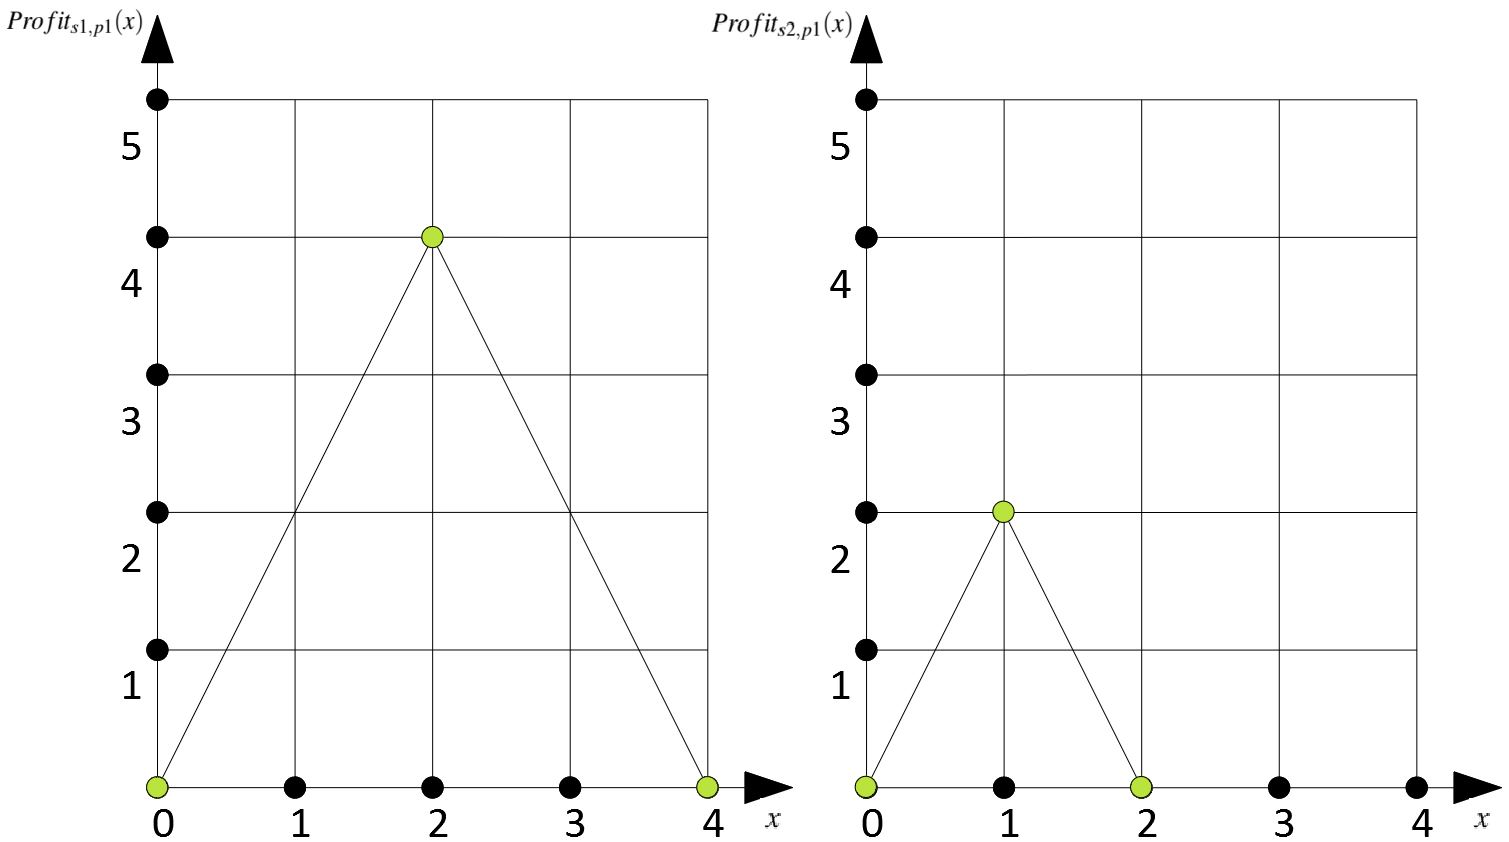
\includegraphics[scale=0.38]{profitsForP1}
\caption{$p_1$ termék profit függvényei $s_1$ és $s_2$ forgatókönyvben}
\label{profit_for_p1}
\end{center}
\end{figure}
A \ref{profit_for_p1}. ábrán láthatóak $p1$ termék profit függvényei.
A bal oldali függvény az $s1$, a jobb oldali az $s2$ forgatókönyvbeli profit függvénye $p1$ terméknek.
Miután ezek a függvények megalkotásra kerültek adott termék összes forgatókönyvére, a következő lépésben ezek beszorzásra kerülnek adott forgatókönyvek valószínűségével.
Ezt a lépést ábrázolja a \ref{profit_for_p1_prob}. ábra.
\begin{figure}
\begin{center}
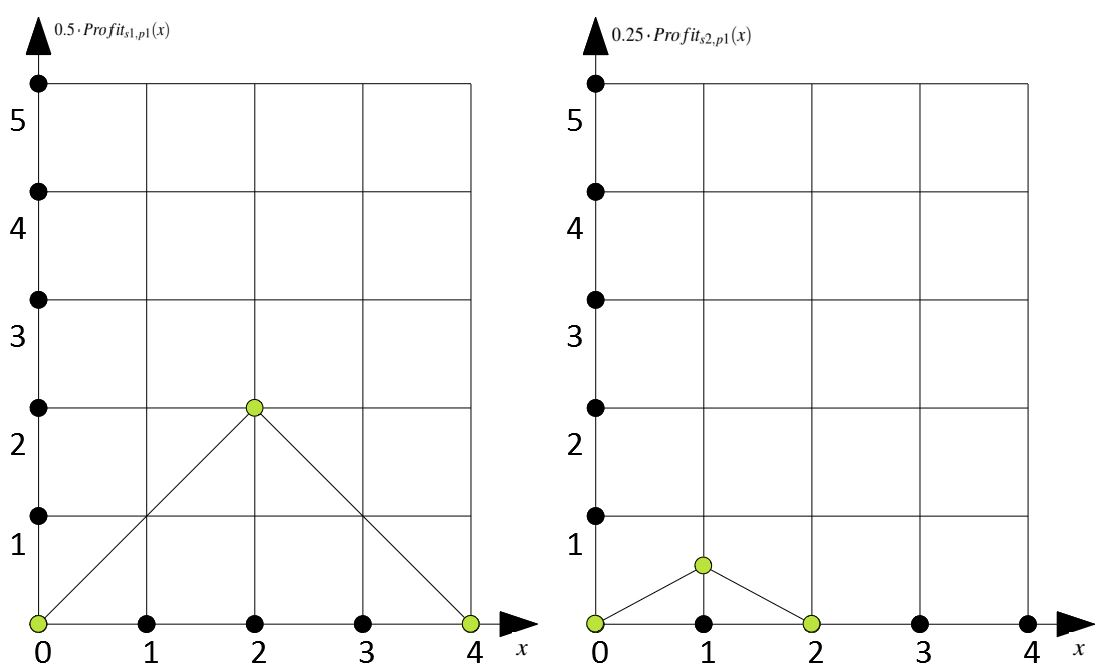
\includegraphics[scale=0.4]{profitsForP1Prob}
\caption{$p_1$ termék összenyomott profit függvényei $s_1$ és $s_2$ forgatókönyvben}
\label{profit_for_p1_prob}
\end{center}
\end{figure}
Ebben a példában $s1$ forgatókönyv valószínűsége $0.5$, $s2$ valószínűsége pedig $0.25$.
Az ábrán látható függvények kiszámításával előáll minden forgatókönyvre a $prob_s \cdot profit_{s,p}$ függvény, amelyeket ezután össze kell adni, hogy előálljon $ExpProfit_{p_1}$ függvény.
Ezt a fenti ábrák alapján előállított $ExpProfit_{p_1}$ függvényt ábrázolja a \ref{expProfit_p1}. ábra.
Miután minden termékre előállításra kerül ez az $ExpProfit_p$ függvény, az $ExpProfit_p(x) \text{ (ahol }x=s_p \cdot b_p)$ értékek összegeként előáll a várható profit.
Azaz minden termék $ExpProfit$ függvényéből lekérdezésre kerül az $x$ értékhez tartozó profit érték, ahol $x$ az adott termékből termelt mennyiség, mely a termelt batchek száma ($b_p$) és azok méretének ($s_p$) szorzataként áll elő.
Jelen esetben a batch méret ($s_p$) egy fixen adott paraméter, hiszen kötött batch méretű esetről beszélünk.
Ezután ezen $ExpProfit_p(x)$ értékek összegzésre kerülnek, ez adja meg a várható profit értékét.
\begin{figure}[H]
\begin{center}
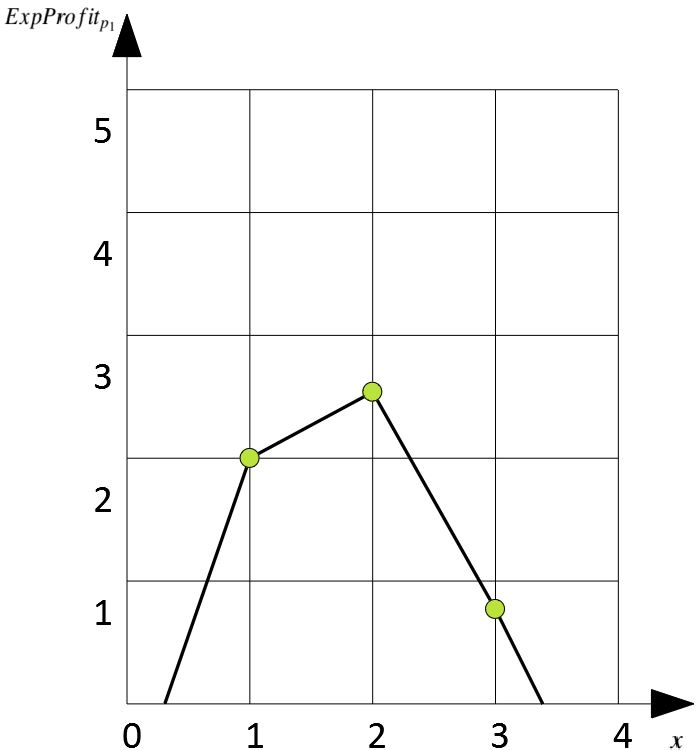
\includegraphics[scale=0.45]{expProfitP1}
\caption{$p_1$ termék ExpProfit függvényének szemléltetése.}
\label{expProfit_p1}
\end{center}
\end{figure}
\subsection{Preventív ütemezés változó batch mérettel} \label{variable_batch_size_modell}
Az ehhez az esethez tartozó lépések megegyeznek az előző kötött batch méretű eset lépéseivel, az $ExpProfit_p$ függvények előállításáig.
Az előző esettel ellentétben azonban, változó batch méret esetén a batch darabszám nem határozza meg egyértelműen az adott termékből termelt mennyiséget. 
Ebben az esetben a batch méretről való döntés is a megoldó algoritmus feladata úgy, hogy $p$ termék batch mérete $s_p^{min}$ és $s_p^{max}$ között legyen.
Mivel ezt a döntést előre meg kell hozni, ezért minden forgatókönyvben azonos méretű lesz minden $p$ termékhez tartozó batch.
Az arról való döntés tehát, hogy adott termékből mennyit gyártsunk, azaz $x_p$ érték meghatározása a következő intervallumból kerül kiválasztásra: $[s_p^{min} \cdot b_p , s_p^{max} \cdot b_p]$.
Ezen érték kiválasztását a \ref{expProfit_func_var}. ábra szemlélteti.
Jelen példában $b_p$ értéke 1, azaz egy darab batchet termelünk $p$ termékből, ezen egy batch termelése mellett a minimális elérhető  termelt mennyiség mennyiség, azaz $b_p \cdot s_p^{min}$ értéke 1.5 kg lesz.
Egy batch termelésével elérhető maximális mennyiség, $b_p \cdot s_p^{max}$ pedig 2.3 kg lesz.
A tartomány amiből tehát ki kell választani x értékét nem más, mint: $[1.5 , 2.3]$, ezt a tartományt jelölik az ábrán a szaggatott vonalak.
Az $x$ optimális értéke úgy kerül kiválasztásra, hogy megnézzük, hogy $ExpProfit_{p1}$ maximális értéke a fenti tartománytól balra, vagy jobbra esik-e, vagy esetleg a tartomány része.
Ha a tartománytól jobbra esik, mint jelen példa szerint, akkor a tartományunk maximális $x$ értéke, azaz jelen esetben $2.3$ kg kerül kiválasztásra, hiszen ezzel az értékkel érhető el jelen tartományban a legnagyobb profit.
Ha a tartománytól balra esne $ExpProfit_{p1}$ maximális értéke, akkor a $[s_p^{min} \cdot b_p , s_p^{max} \cdot b_p]$ tartomány legkisebb értéke, azaz jelen esetben $1.5$ kg kerülne kiválasztásra.
Abban az esetben pedig, ha $ExpProfit_{p1}$ maximális értéke beleesik a $[s_p^{min} \cdot b_p , s_p^{max} \cdot b_p]$ tartományba, akkor a maximális profitot eredményező $x$ érték kerülne kiválasztásra, amely jelen esetben 3 kg lenne.
Az $x_p$ értékek kiválasztása után az összes várható profit a fix batch méretű esettel azonosan módon, $ExpProfit_p(x)$ értékek összegzésével állítható elő. 
\begin{figure}[H]
\begin{center}
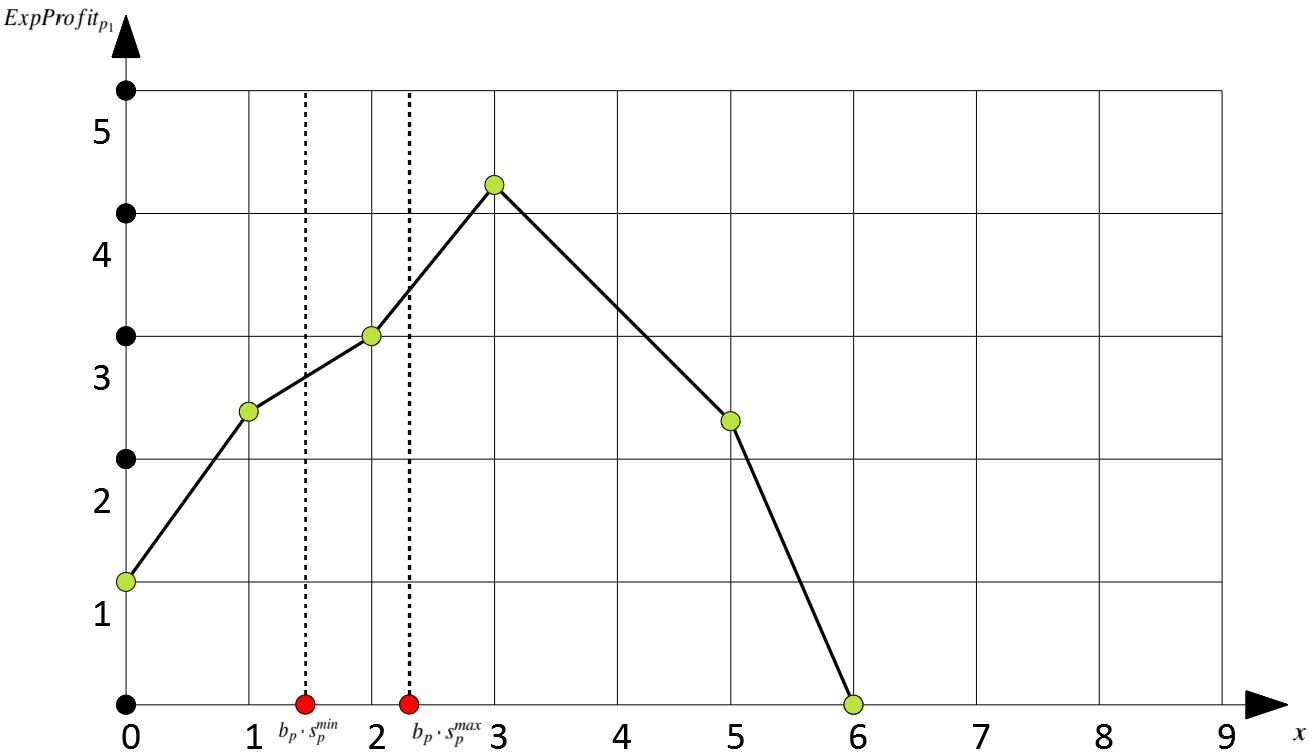
\includegraphics[scale=0.4]{expProfitFuncVar}
\caption{Az optimális $x_p$ érték kiválasztásának szemléltetése}
\label{expProfit_func_var}
\end{center}
\end{figure}
\subsection{Két lépcsős ütemezés (two stage)} \label{TwoStage}
Ebben az esetben $p$ termék gyártandó mennyiségét illető döntés egy bizonytalan esemény bekövetkezése után is meghozható, például, ha egy forgatókönyv már bekövetkezett.
Éppen ezért a termék mennyisége az adott forgatókönyvtől függ, legyen ez: $x_{s,p}$. E mennyiség kiválasztása a következőképpen zajlik:
\begin{equation*}
x_{s,p}(b_p)= \begin{cases}
            b_p \cdot s_p^{max} \quad \text{ha } b_p \cdot s_p^{max}<dem_{s}\\
            dem_{s} \qquad \text{ha } b_p \cdot s_p^{min} \leq dem_{s} \leq b_p \cdot s_p^{max}\\
            b_p \cdot s_p^{min} \quad \text{ ha } b_p \cdot s_p^{min}>dem_{s}
       \end{cases}       
\end{equation*}\\
Látható, hogy a képlet hasonló a \ref{variable_batch_size_modell} pontban bemutatott képlethez, azonban míg ott  az $ExpProfit$ függvényből kerül kiválasztásra az optimális $x_p$ mennyiség (azaz, minden forgatókönyv esetén ez az érték ugyan annyi lesz), addig a két lépcsős ütemezés esetén minden egyes forgatókönyv $Profit$ függvényéből egyenként kerül kiválasztásra az optimális mennyiség.
Azaz a \ref{expProfit_func_var}. ábrán szemléltetett $x$ érték kiválasztása nem az ábrán látható $ExpProfit_p$ függvényből történik, hanem minden, \ref{profit_for_p1}. ábrán látható $profit_{s,p}$ függvényből egyenként történik.
Az így kiválasztott $x$ értékekhez tartozó profit értékek ezután kerülnek beszorzásra a forgatókönyvek valószínűségével.
Az így előállt $(prob_s \cdot Profit(x_{s,p}(b_p))$ értékek ezután kerülnek összegzésre a forgatókönyvekre, majd a termékekre nézve, ezzel áll elő az összes várható profit.
Ezzel megoldható az, hogy egy bizonyos forgatókönyv bekövetkezése után annak elvárásaihoz igazítsuk a termelt batch-ek méretét, jobb várható profitot elérve ezzel a legtöbb esetben.
A várható profit két lépcsős ütemezés esetén tehát a következőképpen számítható ki:
$$\sum_{p \in P} \bigg( \sum_{s \in S}(prob_s \cdot Profit(x_{s,p}(b_p)) \bigg)$$ 
\subsection{Következtetés} \label{piecewise_suggestion}
Az előzőekben bemutatott módszerek ismerete arra enged következtetni, hogy a probléma megoldásához elengedhetetlen az S-gráf keretrendszerben egy olyan osztály definiálása, amely képes  folytonos, szakaszos, lineáris függvények modellezésére, tárolására, azokon történő műveletek végrehajtására. Ezen osztály részletes leírása a \ref{piecewise_class} pontban olvasható.
\section{A PiecewiseLinearFunction osztály} \label{piecewise_class}
Ahogy az már korábban, a \ref{piecewise_suggestion} pontban említésre került, a probléma implementációjához elengedhetetlen egy olyan osztály definiálása, amely kezelni képes folytonos, szakaszos, lineáris függvényeket.
Erre hivatott az általam megalkotott \className{PiecewiseLinearFunction} osztály, amelynek forráskódja \fileName{piecewiselinearfunction.h}, illetve \fileName{piecewiselinearfunction.cpp} fájlokban található a solver \fileName{src\textbackslash base} mappájában.
Egy folytonos, szakaszos, lineáris függvény tárolásához töréspontokat illetve a kezdeti- ,és vég meredekséget kell eltárolni.
Az általam használt függvények eleve tartalmaznak egy törést a kereslet értékénél, hiszen az egyes $profit_{s,p}$ függvények csak a kereslet értékéig növekednek, onnantól pedig vagy beállnak a maximális értékre, ha nincsen felül termelési költség, vagy csökkenni fognak a felültermelési költségek miatt.
Éppen ezért ezen függvények tárolásához elegendő a következő töréspont kiszámítása: $x=dem_{s,p}$, $y=Profit_{s,p}(x)$. 
Majd ezután a kezdeti-, és vég meredekségek a következő képlet segítségével, az alul-, és túl termelési költségek alapján kiszámíthatóak.
\begin{equation*}
Profit_{s,p}(x)= \begin{cases}
            price_{s,p}\cdot x-(dem_{s,p}-x) \cdot uc_{s,p}\qquad \text{ha } x<dem_{s,p} \\
            price_{s,p} \cdot dem_{s,p}-(x-dem_{s,p}) \cdot oc_{s,p}\qquad \text{egyébként}
       \end{cases}
\end{equation*}
Ezek az értékek minden esetben kiszámíthatók, minden forgatókönyv-termék párosra már az input fájl beolvasását követően, hiszen minden sztochasztikus paraméter adott ehhez a fájlban.
Később ezen adatok alapján a többi pont koordinátái, ha valamilyen okból kifolyólag ezek ismerete szükségessé válik, könnyen kiszámíthatóak, hiszen folytonos, lineáris függvényekről beszélünk.
Ezek alapján a \className{PiecewiseLinearFunction} osztály adattagjai a \ref{piecewise_variables}. ábrán láthatóak.
A \ref{piecewise_variables} ábrán látható \className{Coordinate} osztály a függvények töréspontjainak $x$ és $y$ koordinátáinak egyszerű tárolására, lekérdezésére, és összehasonlítására szolgál a megvalósított \textit{setter}, \textit{getter} és felültöltött egyenlőség operátorral.
Ahhoz, hogy a \className{PiecewiseLinearFunction} osztállyal a matematikai modellek minden szükséges művelete elvégezhető legyen, a következő funkcionalitást kell megvalósítani az osztálynak:
\begin{itemize}
\item A függvény skalár értékkel való szorzása
\item A függvény $x$ helyen vett értékének lekérdezése
\item Két függvény összeadása
\item A függvény horizontális nyújtása (a \ref{extended_multiproduct} pontban tárgyalt esetekhez)
\item A függvény maximális értékéhez tartozó koordináták lekérdezése
\end{itemize}
\begin{figure}[H]
\begin{center}
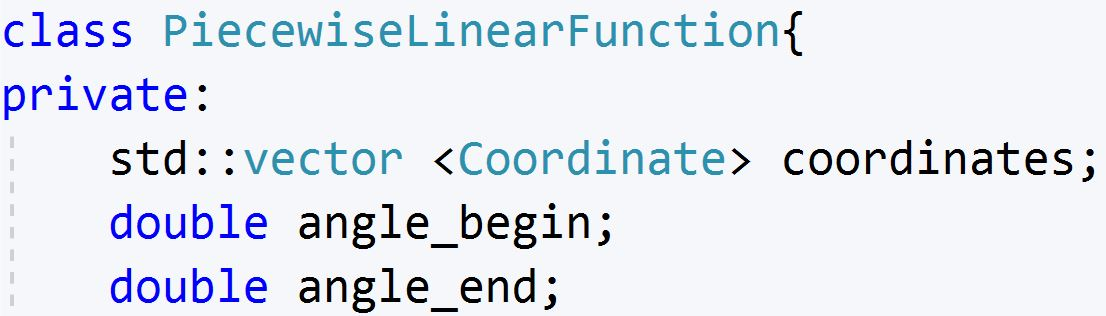
\includegraphics[scale=0.5]{piecewiseVariables}
\caption{A \textit{PiecewiseLinearFunction} osztály adattagjai}
\label{piecewise_variables}
\end{center}
\end{figure}  
\subsection{A függvény skalár értékkel való szorzása} \label{multiplyByScalar}
A függvény skalárral való szorzását a szorzás operátort felültöltő metódus végzi.
Ahhoz, hogy megkapjuk a függvény skalárral való szorzatát, csupán be kell szorozni a \textit{vector}-ban tárolt összes pont $y$ koordinátáját, valamint a kezdeti-, és vég meredekséget a paraméterként kapott $s$-el.
A függvény szorzását szemléltető példa a \ref{profit_for_p1_prob} ábrán látható.
\subsection{A függvény $x$ helyen vett értékének lekérdezése} \label{getValue}
A függvény $x$ helyen vett értékének lekérdezésére a ( ) operátort felültöltő metódus hivatott.
A metódus először is megnézi, hogy a \textit{vector}-ban tárolt koordináta párok között található-e olyan, amelynek $x$ koordinátája egyezik a paraméterként kapott $x$-el.
Ha talál ilyet, egyszerűen visszaadja a megfelelő koordináta páros $y$ értékét.
Ha nem található ilyen pont, akkor annak ki kell számítani a koordinátáit, és hozzá kell adni a \textit{vector}-hoz, majd csak ezután lehet visszaadni a keresett $y$ értéket
Az $x$ értékhez tartozó $y$ érték kiszámítása a keresett $x$ értéke és a \textit{vector}-ban tárolt pontok alapján háromféleképpen történhet:
\begin{itemize}
\item Ha a keresett $x$ értéke kisebb mint a \textit{vector}-ban tárolt első pont $x$ koordinátájának értéke, akkor: 
$y=y_{First}-(x_{First}-x) \cdot Angle_{begin}$ ,ahol $x_{First} \text{ és } y_{First}$ a \textit{vector}-ban tárolt első pont koordinátái.
\item Ha a keresett $x$ érték két a \textit{vector}-ban tárolt pont $x$ koordinátájának értéke közé esik, akkor:
$y=\bigg(\big(x-x_{LastSmaller}\big) \cdot \big((y_{FirstBigger}-y_{LastSmaller})/(x_{FirstBigger}-x_{LastSmaller})\big)\bigg)+y_{LastSmaller}$ ,ahol $x_{LastSmaller} \text{ és } y_{LastSmaller}$ a keresett $x$ értéket megelőző pont koordinátái, míg $x_{FirstBigger} \text{ és } y_{FirstBigger}$ a keresett $x$ értéket követő pont koordinátái. 
\item Ha a keresett $x$ értéke nagyobb, mint a \textit{vector}-ban tárolt utolsó pont $x$ koordinátájának értéke, akkor:
$y=y_{Last}-(x-x_{Last}) \cdot Angle_{end}$ ,ahol $x_{Last} \text{ és } y_{Last}$ a \textit{vector}-ban tárolt utolsó pont koordinátái.
\end{itemize}
\subsection{Két függvény összeadása} \label{addPiecewiseLinearFunction}
Két függvény összeadását az összeadás operátort felültöltő metódus végzi, melynek visszatérési értéke az összegként kapott függvényt tároló új \className{PiecewiseLinearFunction} objektum.
Mivel a függvények tárolásához elegendő három pont tárolása, ezért gyakran előfordul olyan eset, hogy a két összeadni kívánt \className{PiecewiseLinearFunction} objektum nem tartalmazza a szükséges koordinátákat, ezért a hiányzó koordináta párokat először hozzá kell adni, ezt azonban megkönnyíti a \ref{getValue} pontban bemutatott metódus, hiszen elég, ha lekérdezzük az aktuális $x$ értékét mindkét függvény esetén, és ha az valamelyiknél nem található, automatikusan hozzá lesz adva annak pontjaihoz.
Ennek következtében a két függvény összeadása már jóval egyszerűbb feladat.
A fentiek szemléltetésére szolgál a \ref{add_piecewise}. ábra.
A két összeadandó függvényt \textbf{a}-nak, illetve \textbf{b}-nek nevezzük, az összegként adott új függvény pedig a \textbf{c}.
Az ábrán a 90. sorban lekérdezzük \textbf{b} függvény koordinátáit, melyeken a 91. sorban található \textit{for} ciklussal végigiterálunk.
A 92. sorban \textbf{a} függvénynek lekérdezzük x helyen vett értékét, ahol x \textbf{b} függvény soron következő koordinátájának x értéke.
A lekérdezés következtében, ha \textbf{a} függvény eddig nem tartalmazott koordinátát x értékkel, ezen koordináta hozzáadásra kerül a \ref{getValue}. pontban leírtak alapján.
Mivel ezt \textbf{b} függvény minden pontjára megtesszük, ezért a \textit{for} ciklus végeztével \textbf{a} függvény immáron biztosan tartalmazza a \textbf{b} függvényben tárolt összes töréspont x értékéhez tartozó saját x értékű koordinátáit az azon a helyen vett y értékekkel.
Ezután \textbf{a} függvény összes tárolt töréspontján végigiterálunk a 95. sorban található \textit{for} ciklussal.
Ebben a \textit{for} ciklusban létrehozzuk az új \textbf{c} függvény koordinátáit.
Ezen koordináták x értéke az \textbf{a} függvény x értékei lesznek rendre hiszen \textbf{a} immáron tartalmazza az összes közös x értéket \textbf{b}-vel.
A koordináták y értéke pedig $a(x)+b(x)$ lesz.
Mivel a koordináták \methodName{addCoordinate} metódussal való hozzáadása során a kezdeti és a vég meredekségek automatikusan frissítésre kerülnek, ha szükséges ezen értékek újraszámítása, ezért a \textit{for} ciklus végére előálló \textbf{c} függvényben ezeket már nem kell külön beállítani.
A metódus végén pedig visszaadásra kerül az új \textbf{c} összegfüggvény. 
\begin{figure}[H]
\begin{center}
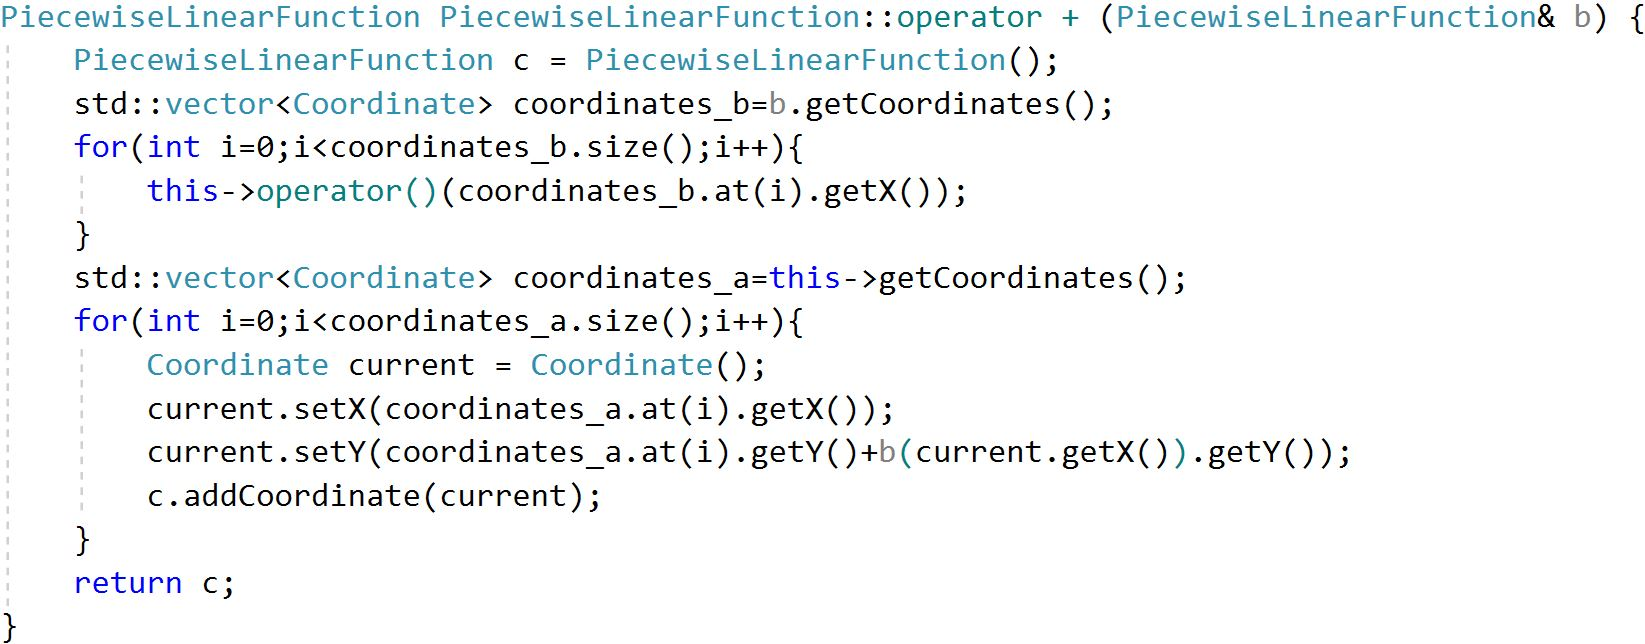
\includegraphics[scale=0.4]{addPiecewise}
\caption{Az összeadást végző metódus}
\label{add_piecewise}
\end{center}
\end{figure}
\subsection{A függvény horizontális nyújtása} \label{stretch}
A függvény a \ref{extended_multiproduct} pontban használt, a \ref{profit_func_stretch} ábrán bemutatott horizontális nyújtását (illetve összenyomását, s értéktől függően) a \methodName{stretchHorizontally(double s)} metódus végzi.
A metódus egyszerűen egy \textit{for} ciklus segítségével a függvény összes pontjának $x$ koordinátáját, valamint a kezdeti-, és vég meredekséget beszorozza a paraméterként kapott $s$ értékkel, illetve a meredekségek esetén annak reciprokával. 
\begin{figure}
\begin{center}
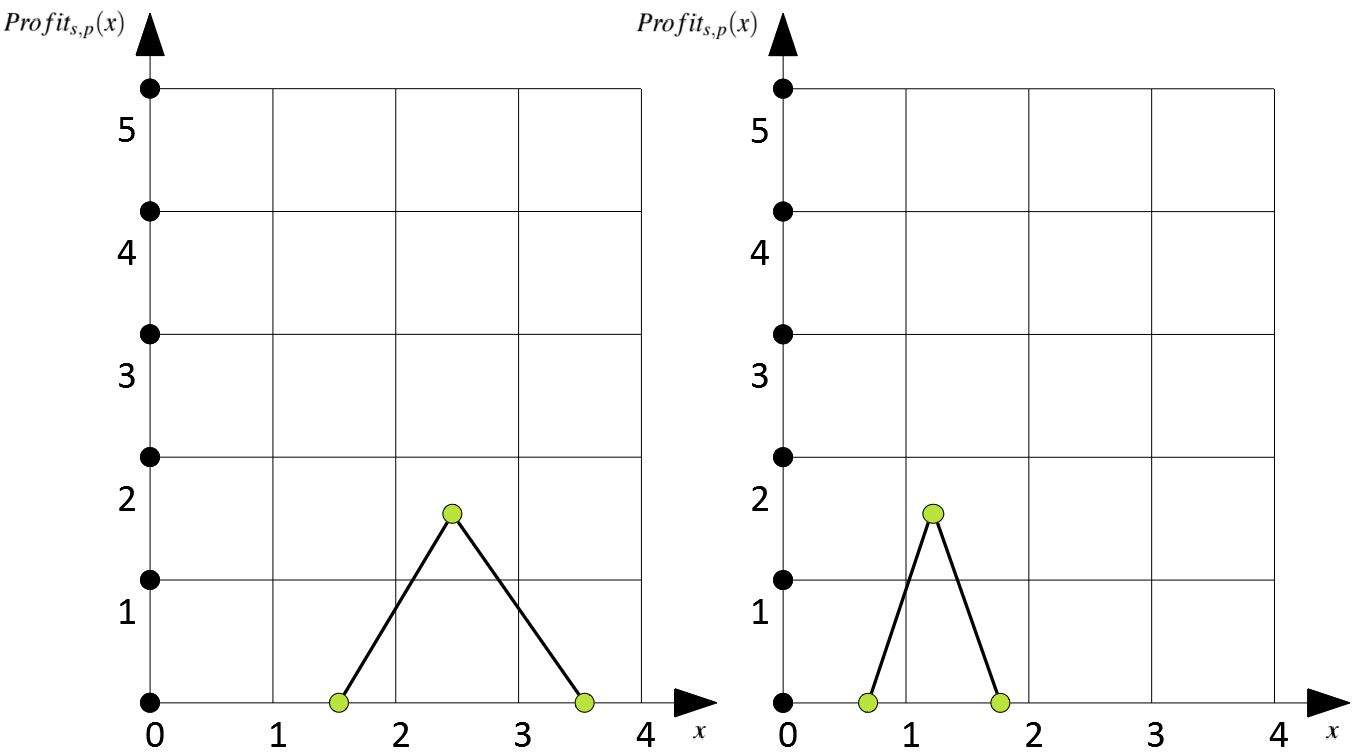
\includegraphics[scale=0.4]{profitFuncStretch}
\caption{Példa a függvény horizontális nyújtására $s=0.5$ értékkel}
\label{profit_func_stretch}
\end{center}
\end{figure}
\subsection{A függvény maximális értékéhez tartozó koordináták lekérdezése}
A függvény maximumának lekérdezését a \methodName{getMaximum()} metódus végzi, mely egy egyszerű maximum keresést valósít meg $y$ koordinátára nézve.
A metódusnak a korábban bemutatott változó batch méretű, illetve két lépcsős esetekben van nagy jelentősége.
\section{Az új paraméterek implementációja}
Ahhoz, hogy az determinisztikus throughput maximalizáló használható legyen a \ref{problem_parameters} pontban bemutatott új sztochasztikus paraméterekkel, fel kell készíteni a megfelelő osztályokat ezen paraméterek kezelésére, be kell olvasni először is ezeket a paramétereket egy input fájlból, majd valamilyen formában le is kell őket tárolni, hogy később a \ref{math_modells} pontban bemutatott műveletek végrehajthatóak legyenek a várható profit kiszámítására.
\subsection{Új kapcsoló definiálása}
Mivel a sztochasztikus throughput maximalizáló működhet preventív, illetve két lépcsős módon, ezért szükségessé vált egy új parancssori kapcsoló bevezetése:
\begin{figure}[H]
\begin{center}
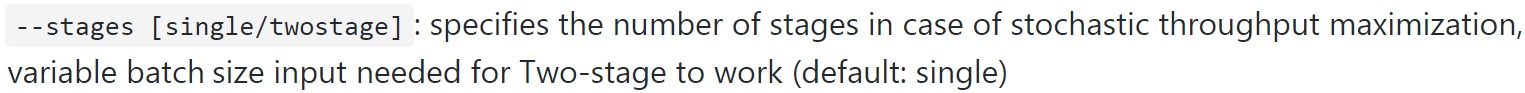
\includegraphics[scale=0.38]{switch}
\caption{Az új kapcsoló leírása a readme fájlban}
\label{switch}
\end{center}
\end{figure}
Abban az esetben, ha nem adjuk meg a kapcsoló értékét, vagy azt single-re állítjuk, preventív módban fog futni az ütemező, ha twostage-t állítunk be, két lépcsős ütemezés fog lefutni, feltéve, hogy a bemeneti fájlban változó batch méretű adatokat adtunk meg.
\subsection{Új input fájl definiálása}
Az általam definiált új input fájl a \fileName{stochastic.ods} a solver \fileName{input} mappájában található.
A fájl lényegében a \fileName{multipurpose.ods} kibővítése a sztochasztikus paraméterekkel.
A \fileName{multipurpose.ods} fájl felépítése a \ref{multipurpose_odshere}. ábrán látható.
\begin{figure}[H]
\begin{center}
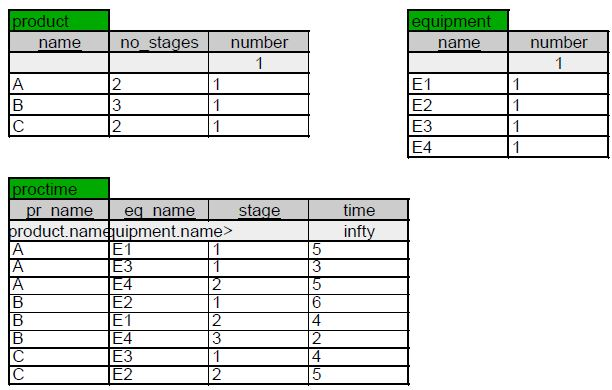
\includegraphics[scale=0.4]{multipurposeOds}
\caption{A \textit{multipurpose.ods} fájl}
\label{multipurpose_odshere}
\end{center}
\end{figure}
A \fileName{stochastic.ods} fájl változtatás nélkül tartalmazza a \fileName{multipurpose.ods} fájl \textbf{equipment}, és \textbf{proctime} tábláit , hiszen ezek tartalmazzák a gépekre, illetve a recept gráfra vonatkozó determinisztikus paramétereket, amelyeket az új esetekben is fel kell használnia a megoldó algoritmusnak.
Ezzel szemben a \textbf{product} tábla a sztochasztikus esetekben nem fogja megállni a helyét, hiszen a batch méretekre vonatkozó adatok hiányoznak belőle, ezeket hozzá kell adni a product táblához.
Ezenkívül a forgatókönyvek adatait is tárolnunk kell, ezért bevezetésre kerültek a\textbf{ scenario}, és a \textbf{scenario\_data} táblázatok, melyek a \ref{problem_parameters} pontban leírt, forgatókönyvekre vonatkozó sztochasztikus adatokat tartalmazzák.
A \fileName{stochastic.ods} fájl felépítése a \ref{stochastic_odshere}. ábrán látható.
\begin{figure}[hbtp]
\begin{center}
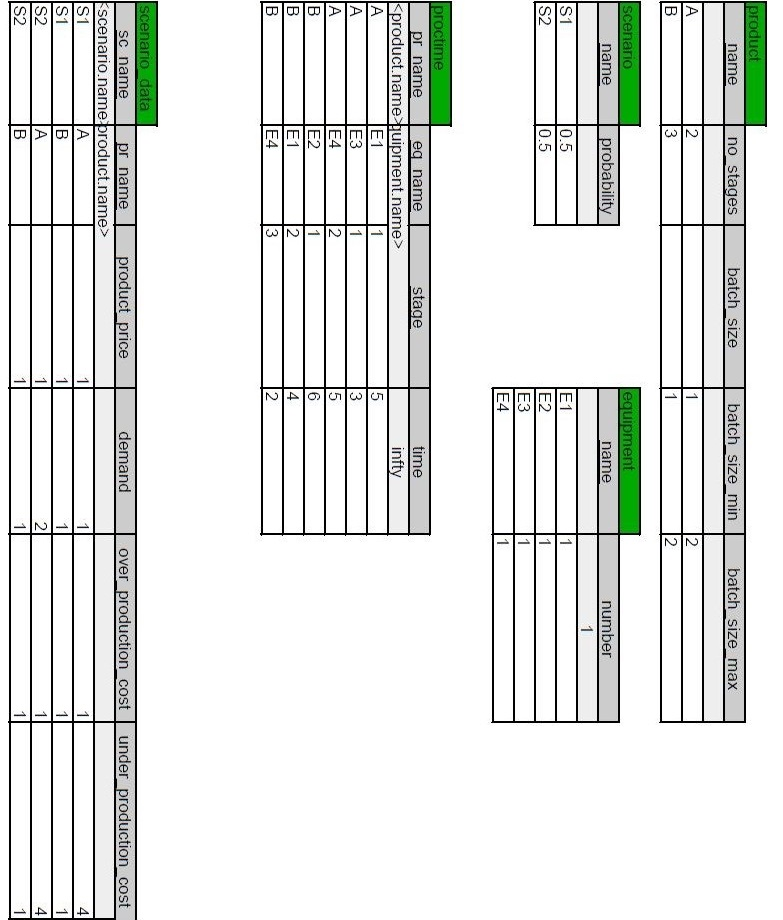
\includegraphics[scale=0.58]{stochasticOds}
\caption{A \textit{stochastic.ods} fájl}
\label{stochastic_odshere}
\end{center}
\end{figure}
\subsection{A fájl beolvasása, beolvasott paraméterek tárolása}
Az input fájl beolvasását a \className{RelationalProblemReader} osztály végzi, melynek feladata a fájlban található paraméterek alapján a recept gráf felépítése, annak visszaadása a \className{MainSolver }osztály számára.
A \className{RelationalProblemReader} először is meggyőződik az input fájl típusáról, majd az alapján sorban beolvassa a megfelelő mezőket az input fájlból.
Éppen azért szükséges egy metódus definiálása, mely képes a sztochasztikus típusú input fájlt megkülönböztetni a többi fajtától.
Ez a metódus az \methodName{IsStochastic()}, illetve a \ref{extended_multiproduct} pontban használt extended input fájl esetén az \methodName{IsExtendedStochastic()}.
Miután meggyőződtünk a fájl sztochasztikus mivoltáról, meghívásra kerül a \methodName{ReadStochastic()} metódus, amely beolvassa, majd eltárolja az \textbf{equipment}, \textbf{product}, \textbf{scenario}, \textbf{scenario\_data}, \textbf{proctime} táblák paramétereit a recept gráfot reprezentáló \className{SGraph} objektum \className{Recipe} objektumában.
Jól látszik, hogy az új sztochasztikus paraméterek tárolásához, a \className{Recipe}, és az \className{SGraph} osztályokban szükséges létrehozni a megfelelő adattagokat, azok eléréséhez szükséges metódusokat.
A termékek batch méretére vonatkozó új paraméterek kezelésére a \className{Product} osztály kiegészítésre került a batch\_size, batch\_size\_min, batch\_size\_max adattagokkal, valamint ide kerülnek letárolásra a \textbf{scenario\_data} tábla adatai is, az erre definiált \className{ScenarioDataEntry} objektumokból álló \textit{vector}-ba.
A \className{ScenarioDataEntry} osztály tartalmazza a \textbf{scenario\_data} táblázatban egy sorában található adatokat, például az adott forgatókönyv azonosítóját, a termék iránti keresletet az adott forgatókönyvben, valamint itt tároljuk le a sztochasztikus paraméterek alapján a \ref{piecewise_class} pontban bemutatott módon létrehozott \className{PiecewiseLinearFunction} objektumot, amely a $Profit_{s,p}$ függvényt reprezentálja.
A fent említett műveleteket, a szükséges objektumok létrehozását a \className{RelationalProblemReader} osztály \methodName{ParseScenarioData} metódusa végzi el.
Ezenkívül bevezetésre került még három \textit{boolean} változó a \className{Recipe} osztályba,  amelyek flag-ként szolgálnak, hogy a throughput maximalizáló könnyen, csupán a \className{Recipe} objektum segítségével meg tudja különböztetni a kötött-, változó batch méretű, és a két lépcsős eseteket.
\section{Szükséges változtatások az S-gráf keretrendszerben} \label{refactor}
A sztochasztikus paraméterek letárolása után nincs más hátra, mint felkészíteni a throughput maximalizálást végző \className{ThroughputSolver} osztályt ezek kezelésére.
Azonban ahhoz, hogy egységesen használható legyen az osztály determinisztikus, illetve sztochasztikus esetben is, némi refaktorálásra volt szükség, ugyanis korábbi állapotában a \className{ThroughputSolver} osztályban találhatóak voltak olyan megoldások, melyek megkövetelték, hogy a profit egyszerűen a $b_p\cdot price_p$ képlettel megkapható legyen, azonban ez a sztochasztikus esetben korántsem ilyen egyszerű.
\subsection{A meglévő kód refaktorálása}
A \className{Throughputsolver} osztály jelenlegi állapotában, determinisztikus esetben kétféleképpen számítja ki a profitot, egyrészt az \className{SGraph} osztály \methodName{GetRevenue()} metódusát használva, másrészt az egyes termékek adatait az \className{SGraph} osztály \className{Recipe} objektumában letárolt \className{Product} objektumok adatait közvetlenül lekérdezve, majd azokat a fent említett $b_p\cdot price_p$ képlettel kiszámítva, és összegezve.
Habár determinisztikus esetben ezek a módszerek megállják a helyüket, ezek jelen állapotban nem túl elegánsak, hiszen a \methodName{GetRevenue()} metódus lényegében ugyan azt a működést éri el, mint az utóbbi közvetlen elérés, és összegzés.
A sztochasztikus esetek bevezetésével ráadásul az adatok közvetlenül a \className{Product} objektumoktól való elérése nem lesz működő módszer, ugyanis ezekben az esetekben a termék paraméterei, ahogy azt már korábban tárgyaltuk, forgatókönyv függőek.
Éppen ezért a sztochasztikus esetekben használt \methodName{GetRevenue()} metódus a \className{Recipe} osztályban kell helyet kapjon, hogy a termék és a forgatókönyv adatok elérése egyaránt lehetséges legyen a metódus számára.
Mivel egy jól karbantartható, hibamentes kódban a fent említett redundanciákat érdemes kiküszöbölni, ezért célszerű lenne a determinisztikus-, és a sztochasztikus esetben használt \methodName{GetRevenue()} metódusok összevonása, mégpedig a \className{Recipe} osztályban, ennek az összevont metódusnak a részletes leírása a \ref{getRevenue} pontban olvasható.
Az összevont \methodName{GetRevenue()} metódus megalkotásának köszönhetően a \className{Throughputsolver} osztály immáron egységes módon kérdezheti le a várható profitot, a probléma milyenségéről való döntés, valamint a profit kiszámítása pedig a \className{Recipe} osztály feladata.
\subsection{A \textit{GetRevenue} metódus} \label{getRevenue}
A \methodName{GetRevenue()} metódus arra szolgál, hogy adott konfiguráció várható összbevételét kiszámítsa, majd visszaadja azt.
A metódus először döntést hoz a probléma típusát illetően a recept objektumban tárolt \textit{boolean} flag segítségével.
Determinisztikus esetben a profit kiszámítása meglehetősen egyszerűen, a \ref{getRevenueNonStoch} ábrán látható módon megtehető. 
\begin{figure}[H]
\begin{center}
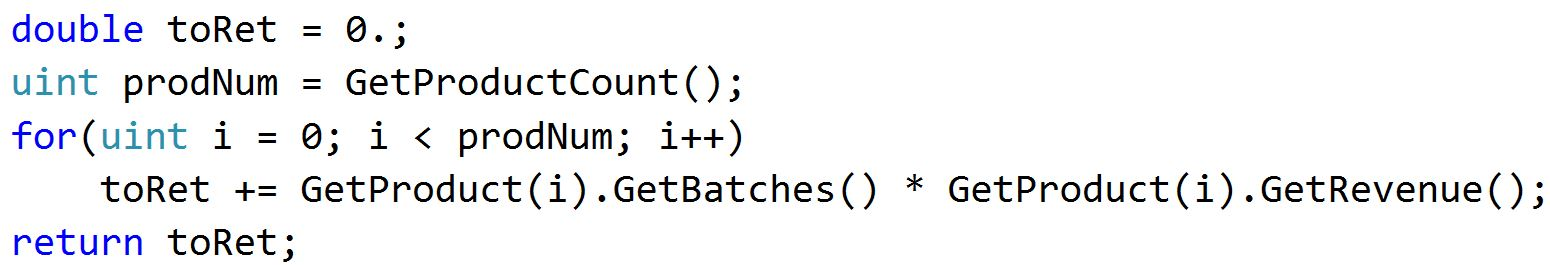
\includegraphics[scale=0.38]{getRevenueNonStoch}
\caption{A \textit{GetRevenue() metódus lefutása determinisztikus esetben}}
\label{getRevenueNonStoch}
\end{center}
\end{figure}
Sztochasztikus esetben is a fenti ábrához hasonló a ciklus, azonban szükség van egy metódusra, amely $x$ számú $p$ termék profitját képes kiszámítani, ez a függvény a \methodName{GetProductRevenue(uint product\_id, uint batches)}.
A metódus megvalósítása közben kiderült továbbá az is, hogy ezenkívül további változtatásokra is szükség van a solver bizonyos karakterisztikái miatt.
A probléma akkor jelentkezik, ha egy adott termékből (legyen ennek neve a példa kedvéért $"A"$) többet termelünk egy batch-nél, ebben az esetben nem az általam várt módon történik a konfiguráció adatainak tárolása.
Ideális számomra az lenne, ha például a konfigurációban két darab $"A"$ batch termelése esetén egy darab $"A"$ termék jelenne meg, és ennek a batch száma $2$ lenne.
Azonban nem ez történik.
A konfigurációban egy $"A"$ és egy $"A\_2"$ nevű termék van jelen egyaránt $1$ batch számmal.
Erre az ütemterv elkészítéséhez van szükség, hogy egyértelműen beazonosíthatóak legyenek az egyes termékek, illetve azok részfolyamatai.
Ez a fajta működés nyilván determinisztikus esetben nem okoz gondot, hiszen ott ekvivalens az, ha két ugyan olyan termékből gyártunk egy-egy darabot, vagy egy termékből kettőt, hiszen a profit értékek nem függenek egymástól, azonban sztochasztikus esetben az alul-, és túl termelési költségek miatt a két eset nem ekvivalens.
Éppen ezért ezt a működést valamilyen formában orvosolni kell.
Erre a problémára nyújt megoldást a \className{Recipe} osztály \methodName{ReduceToBase()} metódusa.
A metódus működéséhez elengedhetetlen, hogy az inputfájlban specifikált termékek neveit elmentsük a \className{Recipe} osztály egy \textit{vector}-ába, a fájl beolvasásakor.
Ezen \textit{vector} terméknevei reprezentálják az úgynevezett "base product"-okat, azaz a kezdeti termékeket.
Ennek a \textit{vector}-nak a birtokában a \methodName{ReduceToBase()} metódus képes az aktuális konfiguráció termékeinek nevét összevetni a kezdeti termékek nevekkel, visszavezetni a konfiguráció termékeit a kezdeti termékekre.
A metódus egy \textit{map}-el tér vissza, amely tartalmazza a kezdeti termékeknek megfeleltetett termékneveket és a hozzájuk tartozó mennyiségeket.
Ha például a konfigurációban a fent említett $"A"$ és $"A\_2"$ termékek szerepelnek egy-egy batch-el, a metódus által visszaadott map tartalma $"A"$ termék lesz kettő batch-el, ezzel kiküszöbölve az említett problémát.

A \methodName{GetRevenue()} metódusnak azonban egy másik, a sztochasztikus esetekkel kapcsolatos problémát is orvosolnia kell.
Ez a probléma a úgynevezett "axial revenue", azaz a tengelyeken számított várható profit értékével kapcsolatos.
Axial revenue-ról akkor beszélünk, ha az adott konfigurációban csupán egy fajta terméket gyártunk, a többi termékből (ha léteznek) ez esetben 0 darabot termelünk.
Ez a sztochasztikus esetekben azért okoz problémát, mert a nem gyártott termékek esetleges alul termelési költségeit le kell vonni az összes profitból, így tehát hiába gyártunk csak egy terméket, a többi termék paraméteri is befolyásolják a várható profitot.
Az alul termelésből eredendő költségek számítása alapvetően nem okozna problémát, hiszen csak ki kellene számolni adott termékek $x=0$ helyen vett $ExpProfit_p(x)$ értékét, és összegezni a kapott értékeket.
Mivel azonban ebben az esetben csak egy fajta terméket termelünk, ezért a konfigurációban csak a termelt termék adatai találhatóak meg, ezért a többi termék $ExpProfit_p(x)$ értékének számítása jelen helyzetben lehetetlen.
Erre azonban megoldást nyújt, ha a korábban említett módon, az inputfájl beolvasását követően a \className{RelationalProblemReader} osztályban nem csak a kezdeti termékek neveit tároljuk el, hanem azok $x=0$ helyen vett $ExpProfit_p(x)$ értékeit is (felhasználva a \ref{getProductRevenue} pontban bemutatott \methodName{GetProductRevenue metódust}).
Ezen értékek tudatában a nem termelt termékekből származó esetleges veszteség immáron levonható az várható profit értékéből, az axial revenue hibátlanul megkapható.

Ezen változtatások segítségével a \methodName{GetRevenue()} függvény ezentúl egységesen használható a \className{ThroughputSolver} osztály számára egy adott konfiguráció összprofitjának kiszámítására, függetlenül a probléma típusától. 
\subsection{A \textit{GetProductRevenue} metódus} \label{getProductRevenue}
A \methodName{GetProductRevenue} metódus hivatott $p$ termék $x$ helyen vett várható profit értékének, azaz $ExpProfit_p(x)$ kiszámítására.
Mivel a metódusnak kezelnie kell a különböző eseteket, ezért szerkezete 4 részre bontható:
\subsubsection{Determinisztikus probléma product revenue számítása}
Determinisztikus esetben a számítás meglehetősen egyszerűen, a $price_p \cdot b_p$ képlettel elvégezhető.
\subsubsection{Kötött batch méretű probléma product revenue számítása}
Kötött batch méretű sztochasztikus esetben a várható profit számítása a \ref{FixBatchSize} pontban leírtak alapján a következő képlettel zajlik: $$\sum_{s \in S} prob_s \cdot profit_{s,p} (s_p \cdot b_p)$$
Először tehát egy \textit{for} ciklus segítségével végigiterálunk az összes forgatókönyvön.
Minden iterációban lekérdezzük az adott forgatókönyvhöz tartozó $profit_{s,p}$ függvényt reprezentáló \className{PiecewiseLinearFunction} objektumot, majd ezt megszorozzuk az aktuális forgatókönyv valószínűségével, hogy előálljon a \ref{profit_for_p1_prob}. ábrához hasonlóan az összenyomott profit függvény.
Ezután ezt hozzáadjuk az $ExpProfit_p$ függvényt reprezentáló \className{PiecewiseLinearFunction} objektumhoz, amely a \textit{for} ciklus előtt került példányosításra.
Miután a ciklus véget ér előáll  $ExpProfit_p$ függvény végleges formája a \ref{expProfit_p1}. ábrához hasonlóan.
Ezután kiszámításra kerül a gyártott mennyiség, azaz az $x$ érték a batch méret és a gyártott batchek darabszámának szorzataként $(s_p \cdot b_p)$.
Kiértékelésre és visszaadásra kerül végül $ExpProfit_p(x)$ értéke.
A kötött batch méretű problémához tartozó forráskód részlete a \ref{fixIMPL}. ábrán látható.
\begin{figure}
\begin{center}
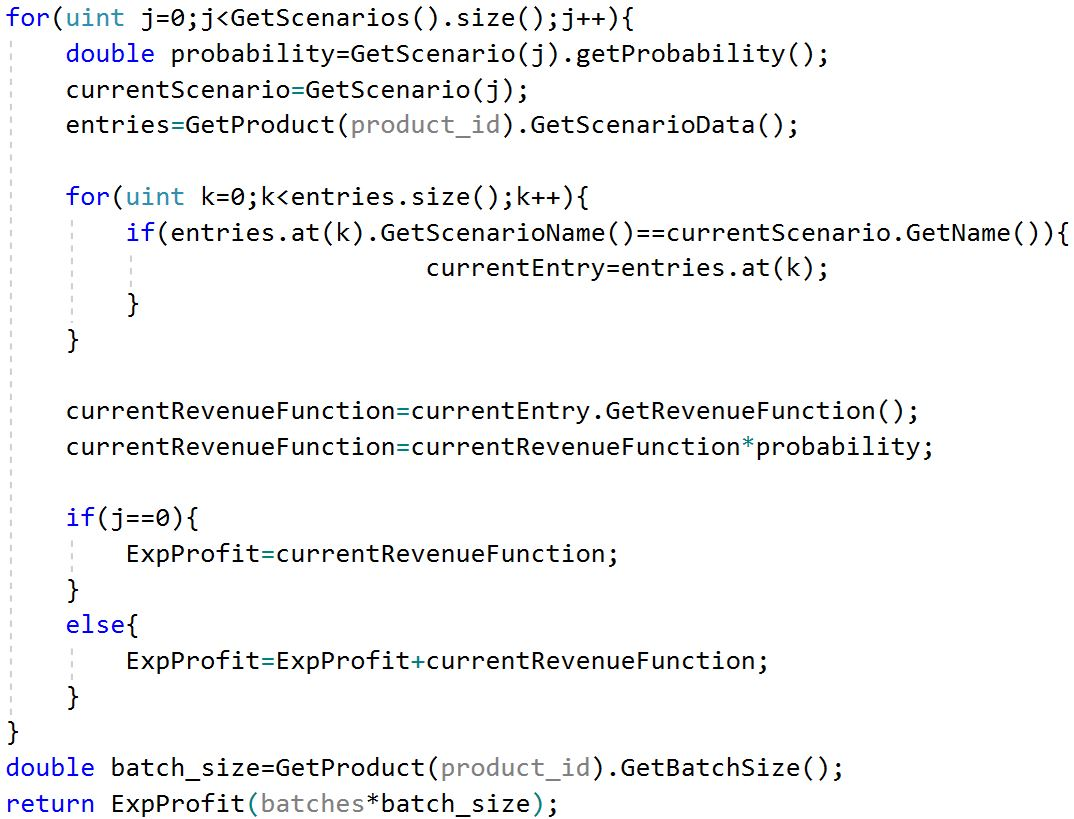
\includegraphics[scale=0.5]{fixIMPL}
\caption{Kötött batch méretű probléma product revenue számítása}
\label{fixIMPL}
\end{center}
\end{figure} 
\subsubsection{Változó batch méretű probléma product revenue számítása}
Változó batch méret esetén a kötött batch méretű esettel azonos módon kapjuk vissza az $ExpProfit_p$ függvényt, tehát a \ref{fixIMPL}. ábrán látható \textit{for} ciklus lefutása ebben az esetben is azonos.
Az $ExpProfit_p$ megkapása után azonban $x$ érték, valamint $ExpProfit_p(x)$ érték kiszámítása a \ref{variable_batch_size_modell}. alfejezetben leírtak alapján, a \ref{expProfit_func_var}. ábrán szemléltetettek szerint történik.
Meghatározásra kerül tehát az  $[s_p^{min} \cdot b_p , s_p^{max} \cdot b_p]$ tartomány, mely segítségével immáron eldönthető az optimális $x$ értéke, és visszaadható a hozzá tartozó  $ExpProfit_p(x)$ érték. 
Ezen folyamat implementációja a \ref{variableIMPL}. ábrán látható.
\begin{figure}
\begin{center}
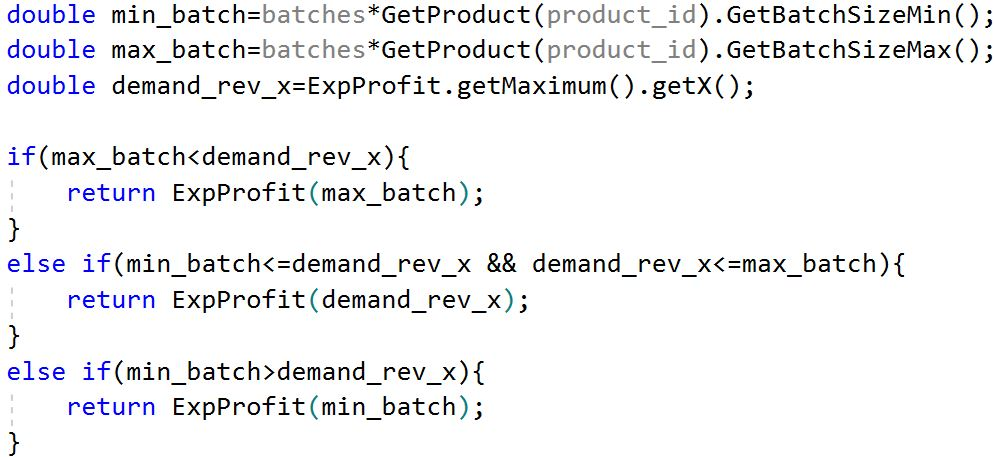
\includegraphics[scale=0.55]{variableIMPL}
\caption{Az optimális profit érték kiszámítása változó batch méret esetén}
\label{variableIMPL}
\end{center}
\end{figure} 
\subsubsection{Két lépcsős probléma product revenue számítása}
Két lépcsős ütemezés esetén a várható profit számítása a \ref{TwoStage} pontban ismertetett módon történik, ezen eset forráskódja a \ref{twostageIMPL}. ábrán látható.
Jól látható, hogy az előző két esettel ellentétben  $ExpProfit_p$ függvény két lépcsős ütemezés esetén nem kerül felépítésre.
A \textit{for} ciklusban az egyes forgatókönyvek $profit_{s,p}$ függvényei segítségével kerül ugyanis kiválasztásra az optimális $x$ érték.
Ezután a $profit_{s,p}(x)$ érték kiértékelésre kerül, majd ezt az értéket megszorozzuk az aktuális forgatókönyv valószínűségével.
Ezen beszorzott profit értékek összegeként áll elő, és kerül visszaadásra jelen termék várható profit értéke.
\begin{figure}[H]
\begin{center}
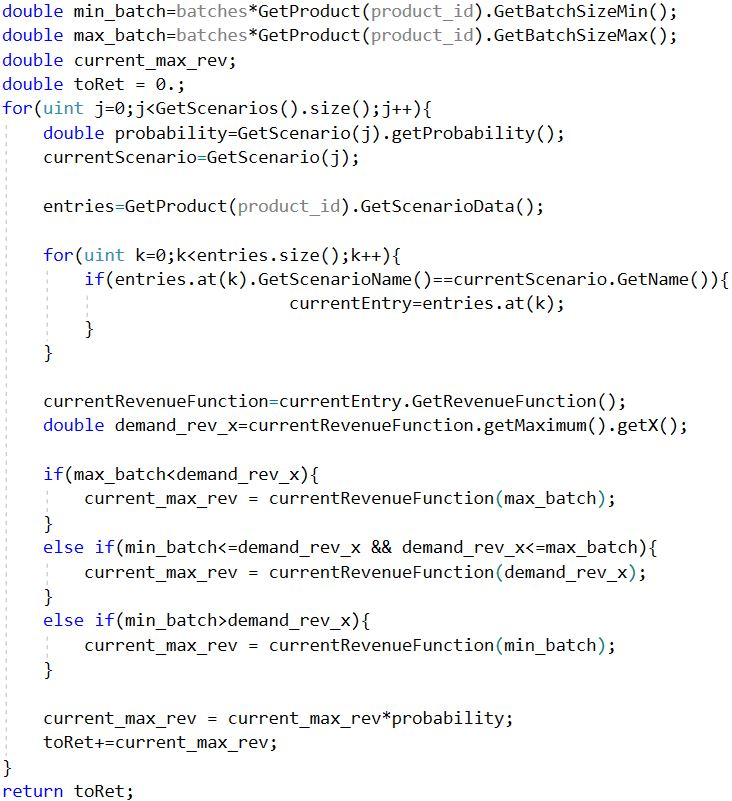
\includegraphics[scale=0.69]{twostageIMPL}
\caption{Két lépcsős probléma product revenue számítása}
\label{twostageIMPL}
\end{center}
\end{figure} 

Ezen módszerek implementációját tartalmazza tehát a \methodName{GetProductRevenue} metódus, amely segítségével ezentúl adott termék profitja, függetlenül a probléma típusától egységesen megkapható.
\subsection{A \textit{Revenue Line} figyelmen kívül hagyása sztochasztikus esetben}
Ahogyan az már a \ref{SgraphProfitMax}. pontban említésre került, a determinisztikus throughput maximalizálóban használatos gyorsítási stratégia az un. Revenue Line, amely lényegében alsó bound-ként szolgál az egyes konfigurációk profitértékeinek összehasonlításához.
A \ref{revLine}. ábrán jól látható, hogy ez a stratégia determinisztikus esetben jó eredménnyel használható, ideális esetben töredékére csökkentheti az ellenőrizendő konfigurációk számát.
Sztochasztikus esetben azonban el kell tekintetnünk a Revenue Line használatától, belátható ugyanis, hogy sztochasztikus esetben ez a vonal nem húzható be, hiszen az azonos revenue értékű konfigurációk nem egy vonalon vannak a sztochasztikus paraméterek értékei miatt, hiszen a determinisztikus esettel szemben itt a revenue értékek nem monoton növekvőek az optimális megoldást tartalmazó téren belül.
Ennek a szemléltetésére szolgál a \ref{revLineStoch}. ábra.
\begin{figure}[H]
\begin{center}
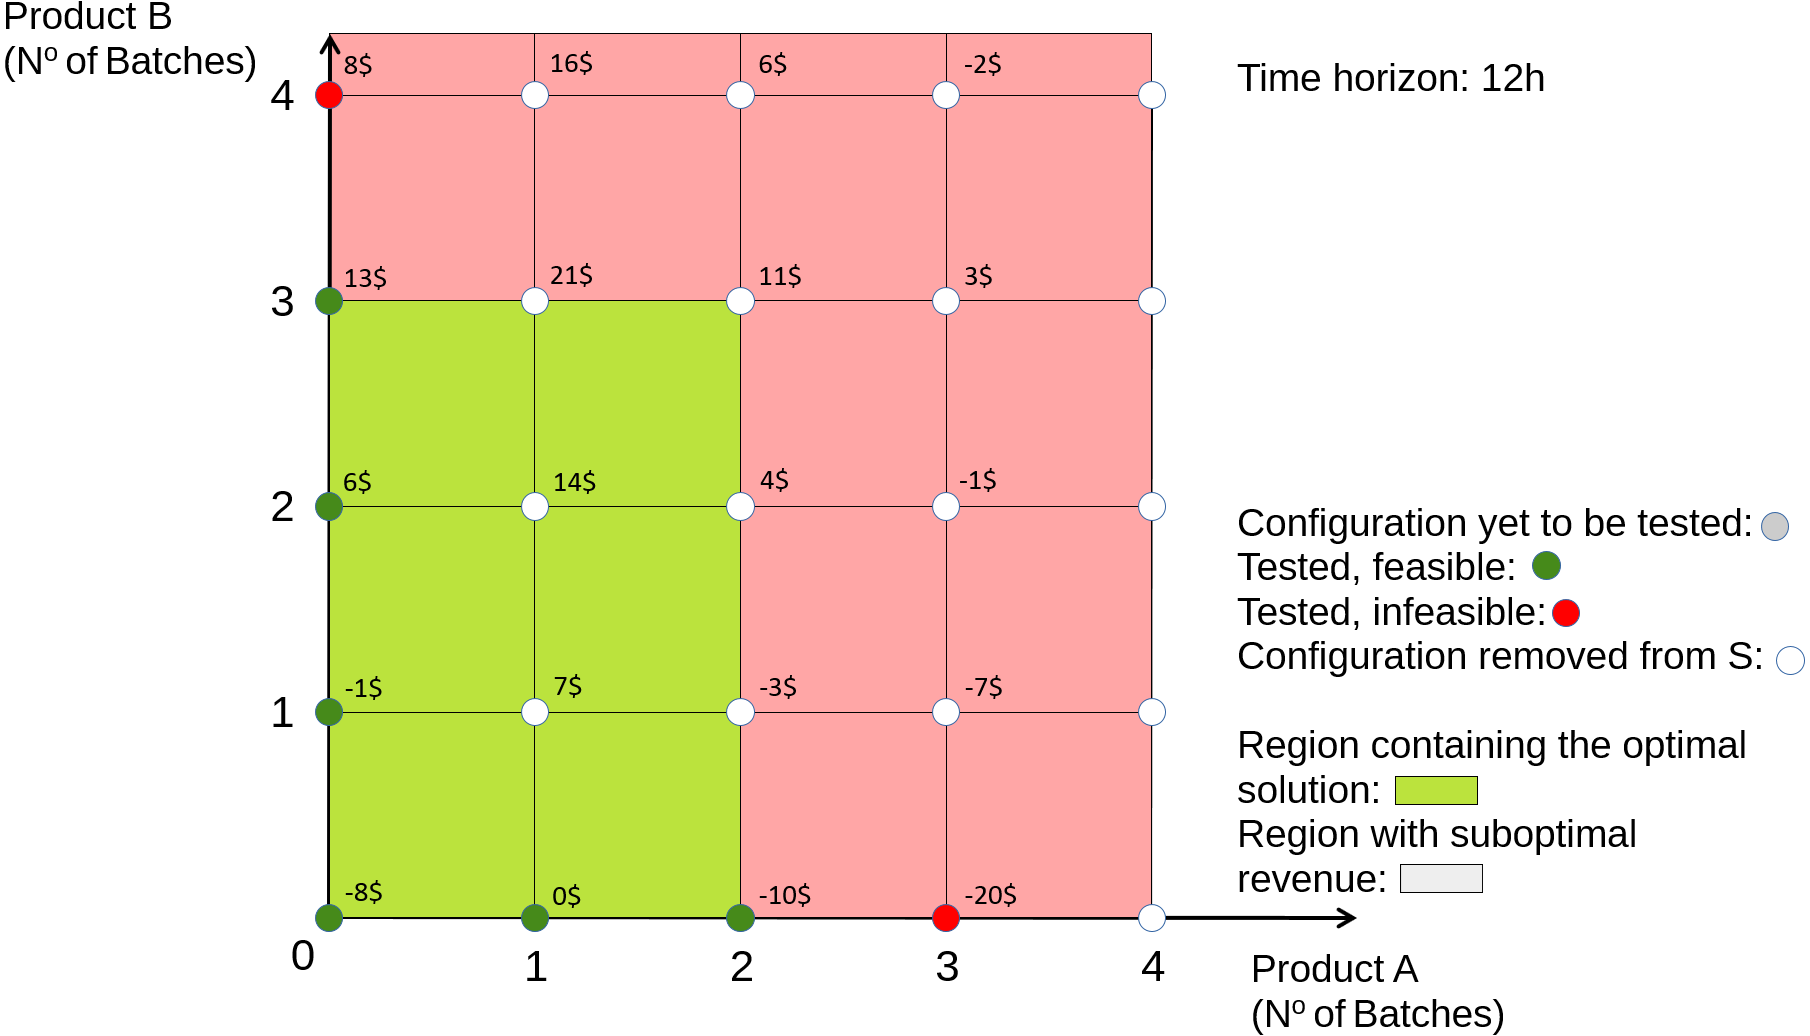
\includegraphics[scale=0.3]{revLineStoch}
\caption{A \textit{Revenue Line} helytelenségének szemléltetése sztochasztikus esetben}
\label{revLineStoch}
\end{center}
\end{figure} 
\subsection{A \textit{ThroughputUI} osztály kiegészítése}
A \className{ThroughputUI} osztály feladata a \className{ThroughputSolver} osztály által kiszámított eredmények megjelenítése a felhasználó számára.
Determinisztikus esetben a Throughput maximalizáló egy példa lefutását a \ref{ThroughputUI} ábra szemlélteti.
\begin{figure}[H]
\begin{center}
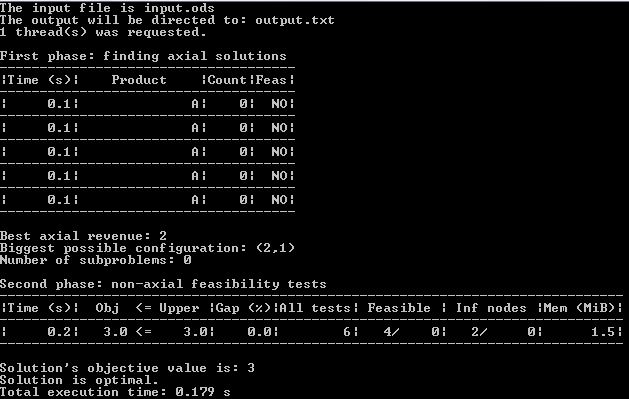
\includegraphics[scale=0.62]{throughputUI}
\caption{Példa a \textit{ThroughputUI} szerkezetére determinisztikus esetben}
\label{ThroughputUI}
\end{center}
\end{figure}
Jól látszik, hogy a \className{ThroughputUI} osztály is kiegészítésre szorul a sztochasztikus esetek kezeléséhez a következőkkel:
\begin{itemize}
\item Optimális batch darabszámok és méretek minden termékre (kötött batch méret és változó batch méret esetén)
\item Optimális batch darabszámok minden termékre, batch méretek minden termék - forgatókönyv párosra (két lépcsős ütemezés esetén)
\item Forgatókönyvek, és a hozzájuk tartozó valószínűségek
\item A várható összprofit értéke forgatókönyvenként
\end{itemize}
Ezen adatok tárolását a \className{ThroughputSolver} osztály általam létrehozott metódusa a \methodName{SaveStochasticStatistics} végzi el felhasználva a \className{ThroughputSolver} osztály \className{Statistics} típusú objektumát, melynek feladata a futás közben a \className{ThroughputUI} osztály számára szükséges statisztikai adatok tárolása.
A \methodName{SaveStochasticStatistics} metódus minden alkalommal lefut, mikor egy új konfiguráció kerül hozzáadásra a \methodName{NewSolution} metódus által.
A sztochasztikus esetek lefutását a \ref{ThroughputUIFixedVar}, és a \ref{ThroughputUITwoStage} ábra szemlélteti.
\begin{figure}[H]
\begin{center}
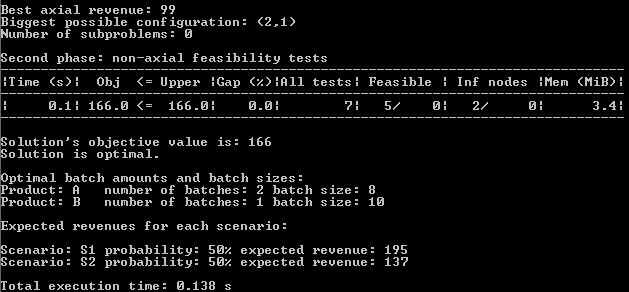
\includegraphics[scale=0.9]{throughputUIFixedVar}
\caption{Példa a \textit{ThroughputUI} szerkezetére kötött, és változó batch méret esetén}
\label{ThroughputUIFixedVar}
\end{center}
\end{figure}
\begin{figure}[H]
\begin{center}
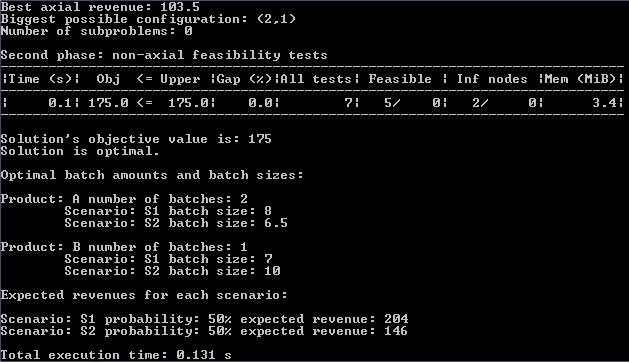
\includegraphics[scale=0.9]{throughputUITwoStage}
\caption{Példa a \textit{ThroughputUI} szerkezetére két lépcsős ütemezés esetén}
\label{ThroughputUITwoStage}
\end{center}
\end{figure}
Mivel az S-gráf keretrendszer throughput maximalizálója alapvetően többszálas működésre lett tervezve, ezért a \className{ThroughputSolver} osztály által használt \className{Statistics} osztály általam bevezetett új adattagjait, illetve azok \textit{getter}, \textit{setter} metódusait fel kell készíteni a párhuzamos használatra.
A C++ programnyelven történő párhuzamos programozás megértéséhez, a szükséges változtatások bevezetéséhez nagy segítségnek bizonyult Anthony A. Williams a témában íródott könyve. \cite{CppConcurrency}
A primitív adattagok esetében az \className{AtomicVariable\textless T\textgreater } osztályt használtam fel, melynek definíciója a solver \fileName{base} mappájában található \fileName{parallel.h} fájlban olvasható.
Az osztály megvalósítja T típusú változó párhuzamos elérését, azon végzett műveletek biztonságos lekezelését \className{Lock} objektumok használatával.
A bonyolultabb adatszerkezetek (például map-ek) párhuzamos elérését a \className{Statistics} osztály \textit{getter}, \textit{setter} metódusaiba implementált \className{Lock} objektumokkal oldottam meg.
A \className{Statistics} osztály általam bevezetett adattagjai a \ref{StatisticsVariables} ábrán láthatóak.
\begin{figure}[H]
\begin{center}
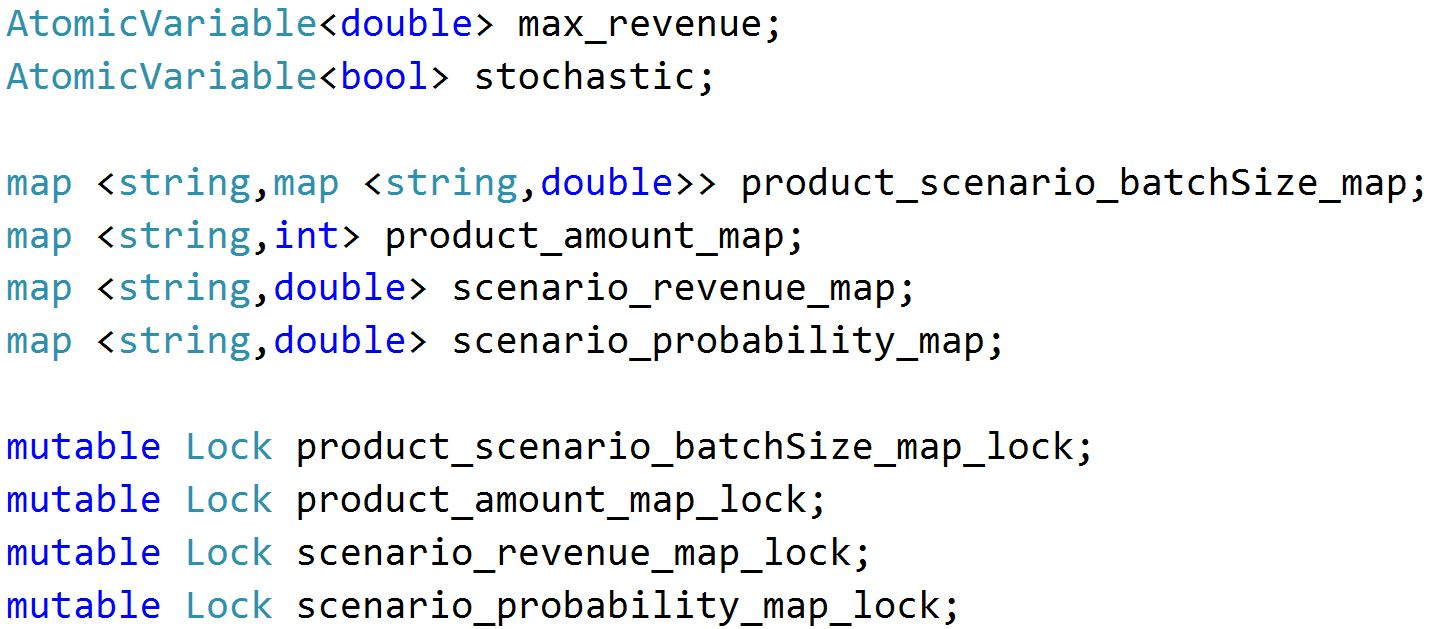
\includegraphics[scale=0.4]{statisticsNewVariables}
\caption{A \textit{Statistics} osztály új adattagjai}
\label{StatisticsVariables}
\end{center}
\end{figure}
Mivel a \textit{map} típusú adattagok \textit{getter} metódusai konstans metódusok, ezzel szemben a solverben definiált \className{Lock} osztály \methodName{Set}, és \methodName{Unset} metódusai nem konstansok, ezért elengedhetetlen volt ez esetben a \className{Lock} típusú objektumok \textit{mutable} kulcsszóval történő definiálása a \className{Statistics} osztályban.
Az általam létrehozott, \className{Lock} objektummal védett \textit{getter}, és \textit{setter} metódusokra példa a \ref{GetterSetterLock} ábrán látható.
\begin{figure}[H]
\begin{center}
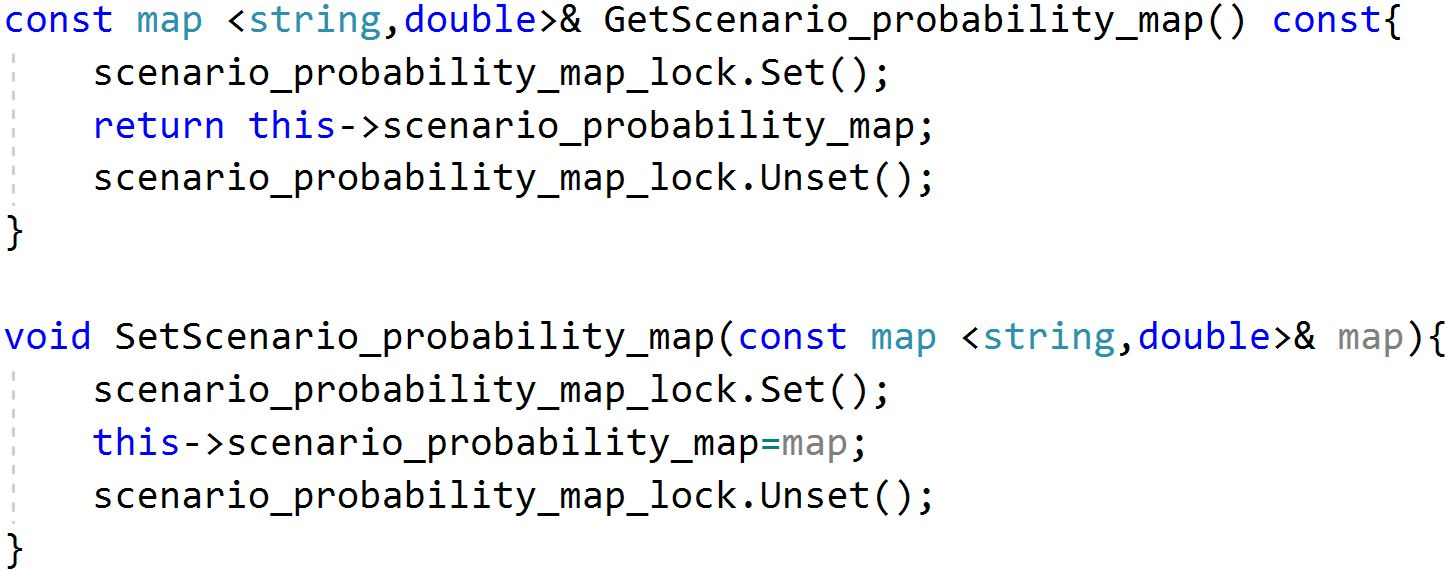
\includegraphics[scale=0.4]{getterSetterLocks}
\caption{Példa a \textit{Lock} objektummal védett \textit{getter}, \textit{setter} metódusokra}
\label{GetterSetterLock}
\end{center}
\end{figure}
\section{Multiproduct receptek esete} \label{extended_multiproduct}
Ebben az alfejezetben tárgyalt esetekben az eddigi feltételezés, miszerint a receptek és a termékek között 1-1 kapcsolat áll fenn, nem teljesül.
Egy recept akár több különböző terméket is előállíthat, illetve egy bizonyos terméket akár több különböző recept is előállíthat.
Az ilyen probléma megoldásához szükséges új fajta input fájlra példa, a \fileName{stochastic\_extended.ods}, amely a \ref{input_files} függelék \ref{stochastic_extended_ods} ábráján látható.
Az ábra alapján jól látható, hogy az előzőekben használt \fileName{stochastic.ods} fájlhoz képest csupán egy új tábla került hozzáadásra, valamint a \textbf{scenario\_data} táblában történt változás.
Ez az egy új hozzáadott tábla a \textbf{sub\_product} nevet kapta, ez hivatott kifejezni a \textbf{product} táblában található receptek által előállított termékeket. \footnote{Mivel a solverben, valamint az eddigi input fájlokban (pl. a multipurpose.ods-ben) is "product" néven hivatkozunk a receptekre, ezért a konzekvenciát megtartandó a receptek által előállított termékek ebben az esetben a "sub product" nevet kapták. A későbbiekben ezen elnevezések egységesítése, refaktorálása a solverben jóval érhetőbb, egységesebb kódot eredményezne, azonban ez túlmutat ezen szakdolgozat témáján.}
A \textbf{sub\_product} tábla tartalmazza az adott receptek által előállított termékek neveit, illetve egy arányszámot, mely megadja, hogy a recept egy batch-ének gyártása során adott termék milyen arányban áll elő.
A \textbf{scenario\_data} táblában pedig immáron a sub product-okra vonatkozó adatok találhatóak a product-ok adatai helyett.
A multiproduct receptekkel kapcsolatos probléma alapvetően két esetre osztható:
\begin{itemize}
\item Az első, egyszerűbb esetről akkor beszélünk, ha egyetlen egy terméket sem eredményez két, vagy több recept.
\item A második, bonyolultabb eset akkor áll fenn, ha egy terméket egyszerre több recept is előállít.
\end{itemize}
Az első eset könnyen megoldható, csupán sorra kell venni az adott recept által gyártott termékek $profit_{s,p}$ függvényeit minden egyes forgatókönyvre, majd a \ref{stretch} pontban bemutatott metódus segítségével a \ref{profit_func_stretch} ábrán látható módon nyújtani azokat a fent említett arányszámmal, mely kifejezi a recept egy batch-e és az előállított termék mennyisége közti arányt.
Miután ezeket a nyújtott függvényeket megkaptuk minden termékre az adott forgatókönyvben, amelyet az adott recept gyárt, ezek összegeként előáll a recept $profit$ függvénye az adott forgatókönyvben.
Ezen $profit$ függvények letárolásával a továbbiakban ez az eset is tekinthető az eredeti sztochasztikus esetnek, az eddig említett módszerek felhasználhatóak a megoldáshoz.
Az egyszerűbb átláthatóság kedvéért azonban célszerű lenne bevezetni pár új jelölést:
\begin{description}
\item[$R$] a receptek halmaza
\item[$P_r$] a termékek halmaza, amelyet $r \in R$ előállít
\item[$s_{r,p}$] az $r \in R$ recept egy batch-e által maximálisan előállítható $p \in P$ termék mennyisége
\end{description}
Az új jelölések alapján $r \in R$ recept $profit$ függvénye az adott forgatókönyvben a következőképpen fejezhető ki:
$$profit_{s,r}=\sum_{p \in P_r} profit_{s,p} \cdot s_{r,p}$$ 
Az előzőeket hivatott megvalósítani a \className{Recipe} osztály általam létrehozott \methodName{CalculateSubProductRevenueSum(uint product\_id)} metódusa, amelyet a \methodName{GetProductRevenue} metódus hív meg abban az esetben, ha érzékeli, hogy multiproduct eset áll fenn.
A metódus lefutása után a probléma a továbbiakban a sztochasztikus alapesetekkel ekvivalens, a várható profit értéke a szokásos módon megkapható.

A második esetben, vagyis amikor fennáll az, hogy egy terméket egyszerre több recept is előállíthat, a probléma megoldása kifinomultabb módszereket igényel, hiszen a receptek várható profitja ebben az esetben nem lesz független egymástól.
Az optimális batch darabszámok, illetve méretek kiszámítására jelen esetben célravezető egy LP modell felírása. \cite{phd_Hegyhati} Az inputfájl definiálásával, illetve a solveren végzett munkámmal megteremtettem ezen eset megoldásának feltételeit is, azonban ennek implementációja túlmutat jelen dolgozat munkáján.
